\documentclass[tikz,border=2pt]{standalone}
\usepackage{amsmath,amssymb}
\usepackage{tikz}

\begin{document}
% An interior point has a whole ball inside E; the interior int(E) is the set of such points
% (the shaded region without its edge).
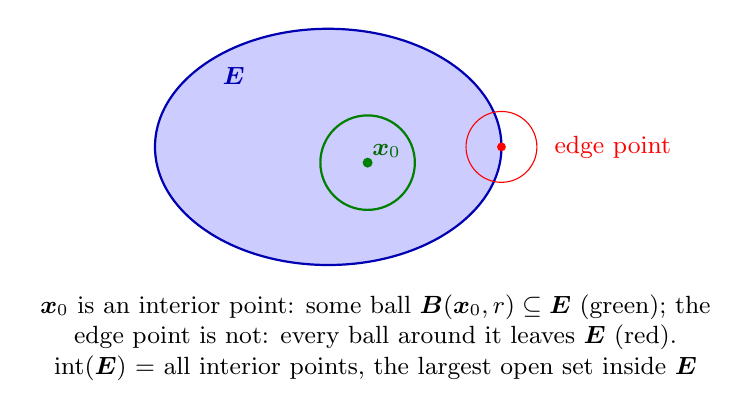
\begin{tikzpicture}[every node/.style={font=\small}]
	\fill[blue!20] (0,0) ellipse (2.2 and 1.5);
	\draw[blue!70!black, thick] (0,0) ellipse (2.2 and 1.5);
	\node[blue!70!black] at (-1.2,0.9) {$\boldsymbol{E}$};
	\fill[green!50!black] (0.5,-0.2) circle (1.8pt) node[above right, inner sep=1.5pt, green!40!black] {$\boldsymbol{x}_0$};
	\draw[green!50!black, thick] (0.5,-0.2) circle (0.6);
	\fill[red] (2.2,0) circle (1.6pt);
	\draw[red] (2.2,0) circle (0.45);
	\node[red, anchor=west] at (2.75,0) {edge point};
	\node[anchor=north, align=flush center, text width=8.6cm] at (0.6,-1.75) {$\boldsymbol{x}_0$ is an interior point: some ball $\boldsymbol{B}(\boldsymbol{x}_0,r)\subseteq\boldsymbol{E}$ (green); the edge point is not: every ball around it leaves $\boldsymbol{E}$ (red). $\operatorname{int}(\boldsymbol{E})$ = all interior points, the largest open set inside $\boldsymbol{E}$};
\end{tikzpicture}
\end{document}
